\documentclass[english,sort&compress]{elsarticle}

%\newcommand{\folder}{/Users/steeve/MA_ZONE/BIBLIO}

% ---------------------------- Packages inclusions.
\usepackage[T1]{fontenc}
\usepackage[utf8]{inputenc}
\usepackage[a4paper]{geometry}
\geometry{verbose}
\usepackage{amsthm,amsmath,amssymb,graphicx,esint,bbm,tabularx,enumitem}
\usepackage{times}%\usepackage{subfloat}
%\usepackage{subfig}
\usepackage{babel}
%\usepackage{calrsfs}

\usepackage{color}\newcommand{\SZ}[1]{{\color{blue} #1}}
\usepackage{color}\newcommand{\jfb}[1]{{\color{red} #1}}
\usepackage{color}\newcommand{\Avoir}[1]{{\color{red}\bf #1}}

% ---------------------------- Pour l'impression et user au mieux la page
\textwidth = 18.5cm
\textheight = 26cm
\oddsidemargin = -1.25cm
\evensidemargin = -1.25cm
\topmargin = -2.25cm

% ---------------------------- Textclass specific LaTeX commands.
\theoremstyle{definition}
\newtheorem{defn}{\protect\definitionname}
\theoremstyle{plain}
\newtheorem{prop}{\protect\propositionname}
\theoremstyle{plain}
\newtheorem{thm}{\protect\theoremname}
\providecommand{\definitionname}{Definition}
\providecommand{\propositionname}{Proposition}
\providecommand{\theoremname}{Theorem}


% ---------------------------- User specified LaTeX commands.
\def\d{\mathrm{d}}
\def\dmu{\mathrm{d}\mu}
\def\fD{\mathcal{D}}
\def\Rset{\mathbb{R}}
\def\X{\mathcal{X}}
%\def\x{\chi}
\def\Y{\mathcal{Y}}
\def\un{\mathbbm{1}}
\def\e{\operatorname{e}}
\def\W{\operatorname{W}}
\def\ext{\operatorname{ext}}
\def\sech{\operatorname{sech}}
\def\arsech{\operatorname{arsech}}
\def\argtanh{\operatorname{argtanh}}
\def\div{\operatorname{div}}
%
\DeclareMathOperator*{\argmax}{\operatorname{argmax}}
%
\newcommand{\Esp}[1]{\mathbb{E}\left[ #1 \right]}
\newcommand{\hypgeom}[2]{\mbox{}_{#1}\hspace{-1pt}F_{#2}}


% ---------------------------- Suppress the footpage
%                              ('preprint submitted to Elsevier' mention)
\makeatletter
\def\ps@pprintTitle{%
  \let\@oddhead\@empty
  \let\@evenhead\@empty
  \def\@oddfoot{\reset@font\hfil\thepage\hfil}
  \let\@evenfoot\@oddfoot
}



% ------------------------ Beginning of the document ------------------------ %
% --------------------------------------------------------------------------- %

\begin{document}


% -------------------------------- Frontpage -------------------------------- %

\title{$\phi$-informational  measures:  some results in a generalized  settings}
%
\author{by jfb \& sz \date{} }
\begin{abstract}
  \Avoir{ To be modified in the light of the new direction of the paper} This paper
  focus on  maximum entropy problems  under moment constraints. Contrary  to the
  usual problem  of finding the  maximizer of a  given entropy, or  of selecting
  constraints such  that a given distribution  is a maximizer  of the considered
  entropy, we consider here the problem  of the determination of an entropy such
  that a given  distribution is its maximizer. Our goal is  to adapt the entropy
  to its maximizer, with  potential application in entropy-based goodness-of-fit
  tests  for  instance. It  allows  us  to  consider distributions  outside  the
  exponential family – to which the  maximizers of the Shannon entropy belong -,
  and also  to consider simple  moment constraints, estimated from  the observed
  sample. Out  approach also  yields entropic functionals  that are  function of
  both probability density  and state, allowing us to  include skew-symmetric or
  multimodal  distributions  in  the  setting. Finally,  extended  informational
  quantities  are  introduced, such  that  generalized  moments and  generalized
  Fisher  informations.  With  thes  extended quantities,  we  propose  extended
  version of the Cram\'er-Rao inequality and of the de Bruijn identity, valid or
  saturated  for   the  maximal   entropy  distribution  corresponding   to  the
  generalized entropy previsouly studied.
\end{abstract}

\maketitle


% ---------------------------------- MaxEnt ---------------------------------- %

\section{Introduction}
\label{sec:Intro}

% Bol96, 98
Since  the  pionner  works of  von  Neuman~\cite{vNeu27},  Shannon~\cite{Sha48},
Boltzmann,  Maxwell,  Planck  and  Gibbs~\cite{Bol64,  Pla15,  Nie52:v2,  Jay65,
  MulMul09} on  the entropy as  a tool  for uncertainty or  information measure,
many investigations were devoted to  the generalization of the so-called Shannon
entropy and its associated  measures~\cite{Ren61, Var66, HavCha67, Csi67, Dar70,
  AczDar75, DarJar79, Tsa88,  Sal87, SalMen93, Sal94, LieVaj06,  Bas13}.  If the
Shannon measures  are compelling,  especially in  the communication  domain, for
compression purposes,  many generalizations  proposed later  on has  also showed
promising   interpretations    and   applications   (Panter-Dite    formula   in
quantification    where     the    R\'enyi    or     Havdra-Charv\'at    entropy
emerges~\cite{PanDit51, Llo82, GerGra92}, codification penalizing long codewords
where the R\'enyi entropy appears~\cite{Cam65,  Ber09} for instance).  The great
majority of  the extended entropies  found in the  literature belongs to  a very
general  class  of  entropic measures  called  $(h,\phi)$-entropies~\cite{Csi67,
  BurRao82, SalMen93,  Sal94, MenMor97, Par06}.   Such a general class  (or more
precisely the subclass of $\phi$-entropies) traced back to the work of Burbea \&
Rao~\cite{BurRao82}. They  offer not only  a general framework to  study general
properties  shared by  special entropies,  but  they also  offer many  potential
applications as  described for instance  in~\cite{Par06}.  Note that if  a large
amount of work deals with divergences, entropies occur as special cases when one
takes a unform reference measure.

 In the settings  of these generalized entropies, the  so-called maximum entropy
 principle takes a  special place.  This principle, advocated  by Jaynes, states
 that  the  statistical distribution  that  describes  a system  in  equilibrium
 maximizes the entropy while satisfying the system's physical constraints (e.g.,
 the  center of  mass, energy)~\cite{Jay57,  Kap89, Arn01,  CovTho06}. In  other
 words, it is the  less informative law given the constraints  of the system. In
 the Bayesian approach, dealing with the stochastic modelisation of a parameter,
 such a principle (or a minimum divergence  principle) is often used to choose a
 prior  distribution  for  the parameter~\cite{Jay68,  Csi91,  Bas13,  FriSri08,
   Rob07}. It also  finds its counterpart in  communication, clustering, pattern
 recognition, problems, among many others~\cite{Kap89, JonByr90, Arn01, HerMa02,
   ParBer09}. In  statistics, some goodness-of-fit  tests are based  on entropic
 criteria  derived   from  the  same   idea  of  constrained   maximal  entropic
 law~\cite{Vas76, Gok83,  Son02, Leq14, Leq15,  GirReg15}. In a large  number of
 works using  the maximum  entropy principle,  the entropy  used is  the Shannon
 entropy, although several extensions exist  in the literature.  However, if for
 some  reason a  generalized entropy  is considered,  the approach  used in  the
 Shannon  case   does  not  fundamentally   change~\cite{KesKap89,  BorLew91:03,
   BorLew91:05, BorLew93}.

%Conversely to the search  for MaxEnt laws, one may wish  to characterize a given
 %probability distribution  as a maximal  entropy distribution.
 One  can consider
the inverse problem which consists in  finding the moment constraints leading to
the  observed distribution  as a  maximal entropy  distribution~\cite{KesKap89}.
Kesavan  \& Kapur  also  envisaged  a second  inverse  problem,  where both  the
distribution and the  moments are given.  The question is  thus to determine the
entropy so that  the distribution is its maximizer. jfb{This  problem has also a
  physical  interpretation, in  the  sense that  the  Shannon entropy  described
  system  in  the  thermodynamic  limit, i.e.,  in  equilibrium,  whereas  other
  entropies are often evoked to describe systems out of equilibrium~\cite{Tsa88,
    TsaMen98,  Tsa99,  Tsa09,  EssSch00,  ParBir05}.}   While  the  problem  was
considered  mainly  in  the  discrete  Shannon  settings  by  Kesavan  \&  Kapur
in~\cite{KesKap89},  we  will  recall  it   in  the  general  framework  of  the
$(h,\phi)$-entropies, and make  a further step considering an  extended class of
these entropies.


While  the  entropy is  a  widely  used  tool  for quantifying  information  (or
uncertainty) attached  to a  random variable or  to a  probability distribution,
other quantities are used  as well, such as the moments  of the variable (giving
information  for instance  on center  of mass,  dispersion, skewness,  impulsive
character), or  the Fisher information.   In particular, the  Fisher information
appears in the context of estimation~\cite{Kay93, Fri04}, in Bayesian inference
through the Jeffrey's  prior~\cite{Rob07, Jef46}, but also  for complex physical
systems  descriptions~\cite{Fri04,   VigBer03,  RomAng99,   RomSan06,  SanGon06,
  TorLop15}.
%\jfb{Among  other  properties,  the  Fisher  information  is  the
%  curvature of  the Kullback-Leibler divergence  between two distributions  of a
%  parametric   family   around   the    parameter   of   the   distribution   of
%  reference~\cite{CovTho06},  describing thus  the  information we  have on  the
%  parameter of reference}.


Although  coming from  different worlds  (information theory  and communication,
estimation, statistics,  physics), these informational quantities  are linked by
well-known  relations  such  the  Cram\'er-Rao's  inequality,  the  de  Bruijn's
identity,  the  Stam's  inequality~\cite{CovTho06, Sta59,  DemCov91,  GuoSha05}.
These relationships have been proved very  useful in various areas, for instance
in communications~\cite{Sta59,  DemCov91, CovTho06},  in estimation~\cite{Kay93}
or in  physics~\cite{FolSit97, Sen11}, among others.  When generalized entropies
are  considered, it  is natural  to question  the other  informational measures'
generalization and the associated identities or inequalities. This question gave
birth  to   a  large  amount   of  work  and  is   still  an  active   field  of
research~\cite{Vaj73,  Boe77,  Ham78,  BoeVan80, BurRao82,  LutYan04,  LutYan05,
  LutYan07, LutLv12, Ber12:06_1, Ber12:06_2, Ber13, Ber13:08}.

In this  paper, we show that  it is possible  to build a whole  framework, which
associates  a  target maximum  entropy  distribution  to generalized  entropies,
generalized moments  and generalized  Fisher information.   In this  setting, we
derive generalized inequalities and  identities relating these quantities, which
are all linked in some sense to the maximum entropy distribution.


\

The paper is organized as  follows. In section~\ref{sec:MaxPhiEnt} we recall the
definition of the generalized $\phi$-entropy.  Thus, we come back to the maximum
entropy   problem   in   this    general   settings.    Following   the   sketch
of~\cite{KesKap89},  we  present a  sufficient  condition  linking the  entropic
functional and  the maximizing distribution,  allowing to both solve  the direct
and the inverse  problems.  When the sufficient conditions  linking the entropic
function and the distribution cannnot be satisfied, the problem can be solved by
introducing  state-dependent  generalized entropies,  which  is  the purpose  of
section~\ref{sec:MultiformEnt}.   In  section~\ref{sec:EscortCR},  we  introduce
informational quantities associated to the generalized entropies of the previous
sections, such that  a generalized escort distribution,  generalized moments and
generalized  Fisher informations.   These  generalized informational  quantities
allow to  extend the  usual informational relations  such that  the Cram\'er-Rao
inequality, relations saturated (or valid) dealing precisely for the generalized
maximum entropy  distribution.  Finally, in section~\ref{sec:deBruijn},  we show
that the  extended quantities allows to  obtain an extended de  Bruijn identity,
profided the distribution  follows a non-linear heat equation.   Some exemple of
determination of  $\phi$-entropies solving  the inverse maximum  entropy problem
are provided  in a  short series of  appendix, showing in  other that  the usual
quantities are recovered in the  well known cases (Gausian distribution, Shannon
entropy, Fisher information, variance).
% to  more exotic  examples.   The paper  ends  then with  some discussions  and
% further directions of investigations and applications.


%------ Ex bout de l'introdution

%The maximal  entropy principle (in  short MaxEnt principle), which  consists in
% searching  maximum entropy  law under  moments constrainst,  is very  usual in
% physics.  The underlying  idea is to determine the  less informative law which
% governs a system (in equilibrium) subject to physical constraints~\cite{Jay57,
%   Kap89, Arn01,  CovTho06}.  Such  an approach finds  also its  counterpart in
% estimation  problems (in communication,  clustering, pattern  recongnition, in
% others) following the  same principle of modeling laws  given some constraints
% and  with   minimal  information~\cite{JonByr90,  Arn01,   HerMa02}.   In  the
% statistics field,  some goodness-of-fit tests  are based on  entropic criteria
% that  sometimes  exploit  the   same  idea  of  constrained  maximal  entropic
% law~\cite{Vas76, Gok83, Son02, Leq14, Leq15, GirReg15}.  The principle of such
% entropy-based tests consist in comparing  the entropy of the tested law, where
% the theoretical  moments are replaced by  their estimates from the  data, to a
% direct estimation of the entropy using the data. As we will see later on, when
% the entropy used is such that the tested law is a maximal entropic law subject
% to the considered moment constraints, the difference of the entropy is nothing
% more than a Bregman divergence, that can be viewed as the distance of a law to
% a reference  law.  In the  same vein, in  estimation domain, when  seeking the
% (likelihood  or   Bayesian)  estimation   of  some  parameters   underlying  a
% parametrized  probability  distribution, if  too  complicated, an  alternative
% approach  is  to  search the  parameters  that  maximize  the entropy  of  the
% law~\cite{Jay68,  Jay82} or  that minimize  a (Bregman,  Csisz\`ar) divergence
% between laws when some {\em a priori} are given~\cite{Csi91, Bas13, FriSri08}.
% %
% To  briefly  come  back  to  the  maximum entropy  principle,  let  $f$  be  a
% probability distribution (of a random  variable $X$) defined with respect to a
% general measure $\mu$ on a set $\X$ and \ $\displaystyle H[f] = - \int_\X f(x)
% \log f(x)  \dmu(x)$ \ be  the Shannon entropy  of $f$.  Subject to  $n$ moment
% constraints  such  as $\Esp{T_i(X)}  =  t_i,  i  = 1  ,  \ldots  , n$  and  to
% normalization, it  is well  known that the  maximum entropy  distribution lies
% within the exponential family, of the form~\cite{Kap89, BorLew91:05, CovTho06,
%   Arn01}
% %
% \[
% f(x) = \exp\left( \sum_{i=1}^n \lambda_i T_i(x) + \lambda_0 \right).
% \]
% %
% Thus, given  constraints, the MaxEnt law  is know, provided  one can determine
% the Lagrangian  parameters $\lambda_i$  insuring the normalization  and moment
% constraints.

% Conversely  to the  search for  MaxEnt laws,  one may  whish to  view  a given
% probability  distribution  as  a   maximal  entropy  distribution  subject  to
% appropriate  constraints.    This  approach  has  interest   for  instance  in
% goodness-of-fit  tests, where  the  law to  be  tested has  to  be the  MaxEnt
% distribution.   Provided  that  the  considered  distribution  belong  to  the
% exponential family,  it is then sufficient  to determine the  set of functions
% $T_i$  adequately~\cite{Gok75,  Kap89,  CovTho06}.   For instance,  the  gamma
% distribution can be viewed as a  maximum entropy distribution if one knows the
% moments $\Esp  X$ and $\Esp{\log(X)}$~\cite{Kap89,  CovTho06, ParBer09, Gok75,
%   Gok83}. A  problem that may arise  for instance in  goodness-of-fit tests is
% the difficulty  to estimate  too complicate moments  and/or to deal  with laws
% outside the  exponential family.  Thus, in  order to extend the  idea of using
% the maximum  entropy distributions  principle, a natural  idea is  to consider
% generalized  entropies~\cite{Ren61, Var66,  HavCha67, Csi67,  Dar70, AczDar75,
%   DarJar79, Tsa88, Sal87,  SalMen93, Sal94, LieVaj06, Bas13}.  As  we will see
% later on,  in such  a generalized context,  the difference of  the generalized
% entropy of the MaxEnt law subject to given moment constraints, and the entropy
% of a  law sharing the  same moments, remains  a Bregman divergence,  which can
% justify ``informationally'' that such an  extension can potentially be used in
% goodness-to-fit  tests.  Moreover, to  impose simple  constraints, it  is very
% natural to  whish to adapt  the entropy to  both the law and  the constraints,
% i.e., to  adapt the entropic  functional to a  fixed law, given  simple moment
% constraints.  This objective is the central part of this paper.

\

In what follows we will define  a series of generalized informational quantities
of  a probability  density that  is defined  with respect  to a  given reference
measure $\mu$  (e.g., the Lebesgue  measure when dealing with  continuous random
variables,   discrete  measure   for  discrete-state   random  variabes,\ldots).
Therefore, rigorously,  all this quantities  depend on the particular  choice of
this reference measure. However, for sake  of simplicity we will omit to mention
this dependence in the notation along the paper.

% ------------------------------ Max (h,phi)-Ent ------------------------------ %

\section{$\phi$-entropies -- direct and inverse maximum entropy problems.}
\label{sec:MaxPhiEnt}

Let  us  first  recall  the   definition  of  the  generalized  $\phi$-entropies
introduced by Csisz\`ar in terms of divergences,  and by Burbea and Rao in terms
of entropies:
%  \SZ{sometimes} known  as entropies  of the
%Salicr\'u's class or of the Csisz\`ar's class:


\begin{defn}[$\phi$-entropy~\cite{BurRao82}]
\label{def:phi-entropy}
Let $\phi: \Y \subseteq \Rset_+ \mapsto \Rset$ be a convex function defined on a
convex  set $\Y$.   Then,  if $f$  is  a probability  distribution defined  with
respect to  a general measure  $\mu$ on a  set $\X \subseteq \Rset^d$  such that
$f(\X) \subseteq \Y$, when this quantity exists,
  %
  \begin{equation}\label{eq:phi-entropy}
    H_{\phi}[f] = - \int_\X \phi(f(x)) \, \dmu(x)
  \end{equation}
  %
  is  the $\phi$-entropy  of  $f$.
\end{defn}
%
The $(h,\phi)$-entropy is defined by $H_{(h,\phi)}[f] = h\left(H_\phi[f]\right)$
where $h$ is  a nondecreasing function.  The definition  is extended by allowing
$\phi$  to be  concave, together  with $h$  nonincreasing~\cite{Csi67, SalMen93,
  Sal94,  MenMor97, Par06}.  If additionnaly  $h$ is  concave, then  the entropy
functional $H_{(h,\phi)}[f]$ is concave.

\

In the  following, since we  are interested by  the maximum entropy  problem and
because $h$  is monotone,  we can  restrict our  study to  the $\phi$-entropies.
Additionnaly,  we will  assume that  $\phi$ is  {\em strictly}  convex and  {\em
  differentiable}.

\

A  useful  related  quantity  to  these  entropies  is  the  Bregman  divergence
associated with convex function $\phi$:
%
\begin{defn}[Bregman divergence and functional Bregman divergence~\cite{Bre67, Bas13}]
\label{def:Bregman}
With the  same assumptions  as in definition~\ref{def:phi-entropy},  the Bregman
divergence associated with $\phi$ defined on a  convex set $\Y,$ is given by the
function defined on $\Y \times \Y$,
  %
  \begin{equation}\label{eq:Bregman}
    D_\phi(y_1,y_2) = \phi(y_1) - \phi(y_2) - \phi'(y_2) \left(y_1-y_2\right).
  \end{equation}
  %
  Applied  to two  functions  $f_i: \X  \mapsto  \Y$, $i=1,  2$, the  functional
  Bregman divergence writes
  \begin{equation}
  \label{eq:FctBregman}
  \fD_\phi(f_1,f_2)  =  \int_\X  \phi(f_1(x)) \, \dmu(x)  -  \int_\X  \phi(f_2(x))
  \, \dmu(x) - \int_\X \phi'(f_2(x)) \left( f_1(x) - f_2(x) \right) \, \dmu(x).
  \end{equation}
  %
  A direct consequence of the strict convexity of $\phi$ is the nonnegativity of
  the   (functional)   Bregman   divergence:   $D_\phi(y_1,y_2)   \ge   0$   and
  $\fD_\phi(f_1,f_2) \ge 0$, with equality if and only if $y_1 = y_2$ and $f_1 =
  f_2$ almost everywhere respectively.
\end{defn}

Note that,  more generally, the  Bregman divergence is defined  for multivariate
convex   functions,    where   the   derivative   is    replaced   by   gradient
operator~\cite{Bre67}.  Extensions for convex  function of functions also exist,
where the derivative is in  the sense of G\^ateau~\cite{NieNoc17}.  Such general
extensions  are not  useful for  our purposes,  thus, we  restrict to  the above
definition where $\Y \subseteq \Rset_+$.


% ------------------------------------------------------------------------------

\subsection{Maximum entropy principle: the direct problem}

Let us  here recall the maximum  entropy problem that consists  in searching for
the distribution maximizing the $\phi$-entropy~\eqref{eq:phi-entropy} subject to
constraints on  some moments $\Esp{T_i(X)}$  with $T_i: \Rset^d  \mapsto \Rset$,
$i=1,\ldots,n$. This direct problem writes
%
\begin{equation}\label{eq:MaxEnt}
\displaystyle f^\star \: = \argmax_{f \in C_t} \left( - \int_\X \phi(f(x))
\, \dmu(x) \right)
\end{equation}
%
with
%
\begin{equation}\label{eq:Ct}
C_t = \left\{ f \ge 0: \: \Esp{T_i(X)} = t_i, i=0,\ldots,n\right\},
\end{equation}
%
where $T_0(x) =  1$ and $t_0 = 1$ (normalization  constraint).  The maximization
problem being strictly concave, the solution  exists and is unique.  A technique
to solve the problem can be to use the classical Lagrange multipliers technique,
but   this  approach   requires  mild   conditions~\cite{KesKap89,  BorLew91:03,
  BorLew93, BenBor92, TebVaj93, Gir97}.  A sufficient condition relating $f$ and
$\phi$ so that $f$  is the desired solution of the problem  is then obtained, as
recalled in the  following proposition.  Below, we prove the  result without the
use of the Lagrange technique.
%, VigHer04,     Ber08,    BerGir15

\begin{prop}[Maximal                                               $\phi$-entropy
    solution~\cite{KesKap89}]
  \label{prop:sol-phi}  Suppose  that  there  exists  a
  probability distribution $f \in C_t$ satisfying
  %
  \begin{equation}\label{eq:sol-phi}
    \phi'\big(f(x)\big) = \sum_{i=0}^n \lambda_i \, T_i(x),
  \end{equation}
  %
  for  some $(\lambda_0,\ldots,\lambda_n)  \in \Rset^{n+1}$.   Then, $f$  is the
  unique solution of the maximal entropy problem~\eqref{eq:MaxEnt}.
\end{prop}
%
\begin{proof}  Suppose that  distribution  $f$ satisfies~\eqref{eq:sol-phi}  and
  consider  any distribution  $g  \in C_t$.  The  functional Bregman  divergence
  between $f$ and $g$ writes
  %
  \begin{eqnarray*}
  \fD_\phi(g,f) & = & \int_\X \phi(g(x)) \, \dmu(x) - \int_\X \phi(f(x)) \, \dmu(x) -
  \int_\X \phi'(f(x)) \left( g(x) - f(x) \right) \, \dmu(x)
  \\[2mm]
  & = & - H_\phi[g] + H_\phi[f] - \sum_{i=0}^n \lambda_i \int_\X T_i(x) 
\left( g(x) - f(x)  \right) \, \dmu(x) \\[2mm]
  & = & H_\phi[f] - H_\phi[g]
  \end{eqnarray*}
   %
  where we  used the fact  that $g$ and  $f$ are both  probability distributions
  with the same  moments $\Esp{T_i(X)} = t_i$.  By  nonnegativity of the Bregman
  functional divergence, we finally get that
  %
  \[
  H_\phi[f] \ge H_\phi[g]
  \]
  %
  for all distribution $g$ with the  same moments as $f$, with equality if and
  only if  $g = f$ almost  everywhere.  In other  words, this shows that  if $f$
  satisfies~\eqref{eq:sol-phi}, then it is the desired solution.
\end{proof}

Hence,  given  an entropic  functional  $\phi$  and moments  constraints  $T_i$,
eq.~\eqref{eq:sol-phi}  leads the  the maximum  entropy distribution  $f^\star$.
This distribution  is parametrized by  the $\lambda_i$ or, equivalently,  by the
moments $t_i$.
%;  these  factors are related by the moments $t_i$.

Note  that  the reciprocal  is  not  necesarilly  true,  as shown  for  instance
in~\cite{BorLew93}.   However,  the   reciprocal  is   true  when   $\X$  is   a
compact~\cite{Gir97} or for any $\X$ provided  that $\phi$ is locally bounded on
$\X$~\cite{Gir07}.




% ------------------------------------------------------------------------------

\subsection{Maximum entropy principle: the inverse problems}

As stated  in the introdution,  two inverse  problems can be  considered started
from a  given distribution $f$.   These problems  were considered by  Kesavan \&
Kapur in~\cite{KesKap89} in the discrete framework.

\

The first inverse problem consists in searching for the adequate moments so that
a  desired distribution  $f$  is the  maximum entropy  distribution  of a  given
$\phi$-entropy. A solution  can thus consist in identifying  functions $T_i$ and
coefficients $\lambda_i$ in order  to satisfy eq.~\eqref{eq:sol-phi}. Obviously,
this is not always an easy task, and even not always possible.  For instance, it
is  well  known that  the  maximum  Shannon  entropy distribution  given  moment
constraints   fall  in   the  exponential   family~\cite{CovTho06,  BorLew91:05,
  Arn01}. Therefore, if $f$  does not belong to this family,  the problem has no
solution.

\

The second  inverse problem consists  in designing  the entropy itself,  given a
target  distribution  $f$  and  given  the  $T_i$.   In  other  words,  given  a
distribution  $f$, eq.~\eqref{eq:sol-phi}  may allow  to determine  the entropic
functional $\phi$ so that $f$ is its maximizer.

As  for the  direct problem,  in  the second  inverse problem,  the solution  is
parametrized by the $\lambda_i$. Here,  required properties on $\phi$ will shape
the  domain the  $\lambda_i$ live  in. In  particular $\phi$,  must satisfy  the
following properties:
%
\begin{itemize}
\item the  domain of definition  of $\phi'$ must  include $f(\X)$; this  will be
  satisfied by construction.
%
\item from  the strict  convexity property of  $\phi$, $\phi'$ must  be strictly
  increasing.
\end{itemize}
%
Hence,  because $\phi'$  must  be  stricly increasing,  its  clear that  solving
eq.~\eqref{eq:sol-phi}  requires the following two conditions:
%
\begin{enumerate}[label=(C\arabic*)]
\item\label{MonotonyDomains:cond}   $f(x)$   and   $\displaystyle   \sum_{i=1}^n
  \lambda_i  \, T_i(x)$  must  have the  same  variations, i.e.,  $\displaystyle
  \sum_{i=0}^n   \lambda_i  \,   T_i(x)$  is   increasing  (resp.    decreasing,
  resp. constant) where $f$ is increasing (resp. decreasing, resp. constant).
%
\item\label{LevelSets:cond} $f(x)$ and  $\displaystyle \sum_{i=1}^n \lambda_i \,
  T_i(x)$ must have the same level  sets, $f(x_1) = f(x_2) \: \Leftrightarrow \:
  \displaystyle \sum_{i=0}^n  \lambda_i \, T_i(x_1) =  \sum_{i=0}^n \lambda_i \,
  T_i(x_2)$
\end{enumerate}
%
%  i.e.,  $\forall  (x_1,x_2)  \in  \X^2,  \quad  f(x_1)  \le  f(x_2)  \:
%\Leftrightarrow  \:   \displaystyle  \sum_{i=0}^n  \lambda_i   \,  T_i(x_1)  \le
%\sum_{i=0}^n \lambda_i \,  T_i(x_2)$. 
For instance, in the univariate case, for one moment constraint, %negative, then
%
\begin{itemize}
\item for $\X = \Rset_+, \: T_1(x) = x$, $\lambda_1$ must be negative and $f(x)$
  must be decreasing,
%
\item for $\X = \Rset, \: T_1(x) = x^2$ or $T_1(x) = |x|$, $\lambda_1$ must be
  negative and $f(x)$ must be even and unimodal.
\end{itemize}

\

Under  conditions~\ref{MonotonyDomains:cond} and~\ref{LevelSets:cond}, the
solutions of eq.~\eqref{eq:sol-phi} are given by
%
\begin{equation}\label{eq:derivative-phi}
\phi'(y) = \sum_{i=0}^n \lambda_i \, T_i\!\left(f^{-1}(y)\right)
\end{equation}
%
where $f^{-1}$ can be multivalued.

\

Eq.~\eqref{eq:sol-phi}  provides   an  effective   way  to  solve   the  inverse
problem. However,  there exist situations  where there do  not exist any  set of
$\lambda_i$ such that conditions \ref{MonotonyDomains:cond}-\ref{LevelSets:cond}
are satisfied (e.g., $T_1(x)  = x^2$ with $f$ not even).  In such  a case, a way
to  go  is   to  extent  the  definition  of  the   $\phi$-entropy,  purpose  of
section~\ref{sec:MultiformEnt}.
%Before, we present briefly three examples.}


% ------------------------------------------------------------------------------

\subsection{Second inverse maximum entropy problem: some examples}

To  illustrate  the previous  subsection,  let  us  analyze very  briefly  three
examples: the  very famous Gaussian  distribution (example 1),  the $q$-Gaussian
distribution also intensively  studied (example 2) and  the arcsine distribution
(example  3),  both three  with  a  second  order moment  constrainst.   \SZ{The
  Gaussian, $q$-Gaussian, and arcsine distributions  will serve as a a guideline
  all along  the paper.}  The  details of the  calculus, together with  a deeper
study related to the  sequel of the paper, are rejected  in the appendix.  Other
examples are also given in this  appendix. In both three examples, \SZ{except in
  the next  section}, we consider the  second order moment constraint  $T_1(x) =
x^2$.

\begin{description}%[label= Example~\alph*]
\item[Example~1]  The  Gaussian  distribution $f_X(x)  =  \frac{1}{\sqrt{2  \pi}
  \sigma} \exp\left(  - \frac{x^2}{2  \, \sigma^2} \right)$  defined over  $\X =
  \Rset$, with the constraint $T_1(x) =  x^2$ viewed as a maximum $\phi$-entropy
  imposes  that  $\lambda_1  <  0$.    Rapid  calculus  leads  to  the  entropic
  functional,   after  a   reparametrization  of   the  $\lambda_i$'s,   of  the
  form, $$\phi(y) = \alpha \, y \log(y)  + \beta \, y + \gamma \quad \mbox{with}
  \quad \alpha > 0,$$  that is nothing more than the Shannon  entropy, up to the
  scaling factor $\alpha$, and a shift  (except for $\gamma = -\beta$). One thus
  recovers the  long outstanding fact that  the Gaussian is the  maximum Shannon
  entropy distribution with the second order moment constraint.
%
\item[Example~2]   The  $q$-Gaussian   distribution,  also   known  as   Tsallis
  distribution,   $f_X(x)  =   C_q   \left(  1   -  (q-1)   \frac{x^2}{\sigma^2}
  \right)_+^{\frac{1}{1-q}}$, where $q > 0, \: q  \ne 1, \: x_+ = \max(x,0)$ and
  $C_q$ is  the normalization coefficient, defined  over $\X = \Rset$,  with the
  constraint $T_1(x) = x^2$ viewed as a maximum $\phi$-entropy imposes also that
  $\lambda_1 <  0$.  Rapid calculus  leads to  the entropic functional,  after a
  reparametrization   of  the   $\lambda_i$'s,   as,  $$\phi(y)   =  \alpha   \,
  \frac{y^q-y}{q-1} + \beta \, y +  \gamma \quad \mbox{with} \quad \alpha > 0,$$
  that     is     nothing     more    than     the     Havrdat-Charv\'at-Tsallis
  entropy~\cite{HavCha67,  Dar70, Tsa88,  CosHer03},  up to  the scaling  factor
  $\alpha$, and  a shift \SZ{(except for  $\gamma = -\beta$)}.  One  recover the
  also well  known fact  that the  $q$-Gaussian is  the maximum  Shannon entropy
  distribution with the second  order moment constraint~\cite{CosHer03}.  In the
  limit case  $q \to 1$, the  distribution $f_X$ tends to  the Gaussian, whereas
  the Havrdat-Charv\'at-Tsallis entropy tends to the Shannon entropy.
%
\item[Example~3] The  arcsince distribution,  $f_X(x) = \frac{1}{\pi  \sqrt{2 \,
    \sigma^2 - x^2}}$, defined  over $\X = \left( -\sigma \sqrt2  \, ; \, \sigma
  \sqrt2  \right)$, with  the  constraint $T_1(x)  = x^2$  viewed  as a  maximum
  $\phi$-entropy imposes  now that $\lambda_1 >  0$. Short algebra leads  to the
  entropic functional, after a reparametrization of the $\lambda_i$'s, $$\phi(y)
  = \frac{\alpha}{y} + \beta \, y + \gamma \quad \mbox{with} \quad \alpha > 0.$$
  This entropy is non usual and, due to its form, is potentially finite only for
  densities  defined over  a  bounded  support and  that  are  divergent in  its
  boundary (integrable divergence).
\end{description}




% ------------------------- State-dependent Entropies ------------------------ %

\section{State-dependent entropic functionals and mimization revisited}
\label{sec:MultiformEnt}

In order to follow asymmetries of  the distribution $f$ and adress the limiation
raised above, an idea  is to allow the entropic functional to  be depend also on
the state variable $x$:
%
\begin{defn}[State-dependent $\phi$-entropy]\label{def:asym_phi-entropy}
  Let $\phi: \X \times  \Y \mapsto \Rset$ such that for any  $x \in \X \subseteq
  \Rset^d$, function $\phi(x,\cdot)$  is a convex function on  the closed convex
  set  $\Y \subseteq  \Rset_+$.   Then,  if $f$  is  a probability  distribution
  defined with  respect to  a general measure  $\mu$ on  set $\X$ and  such that
  $f(\X) \subseteq \Y$,
  %
  \begin{equation}\label{eq:asym_phi-entropy}
    H_\phi[f] = - \int_\X \phi(x,f(x)) \, \dmu(x)
  \end{equation}
  %
  will be  called state-dependent $\phi$-entropy of  $f$.  Since $\phi(x,\cdot)$
  is convex, then the entropy functional $H_\phi[f]$ is concave.
  %
  A particular case arises when, for  a given partition $(\X_1 , \ldots , \X_k)$
  of $\X$, functional $\phi$ writes
  %
  \begin{equation}\label{eq:multiform_phi-entropy}
    \phi(x,y) = \sum_{l=1}^k \phi_l(y) \un_{\X_l}(x)
  \end{equation}
  %
  where $\un_A$ denotes the indicator of set $A$.  This functional can be viewed
  as a ``$(\X_1 , \ldots , \X_k)$-extension'' over $\X \times \Y$ of a multiform
  function  defined on  $\Y$,  with  $k$ branches  $\phi_l$  and the  associated
  $\phi$-entropy   will   be  called   $(\X_1   ,   \ldots  ,   \X_k)$-multiform
  $\phi$-entropy.
\end{defn}

\

As in  the previous  section, we restrict  our study to  functionals $\phi(x,y)$
{\em strictly convex and differentiable} versus $y$.

\

Following  the  lines  of  section~\ref{sec:MaxPhiEnt},  a  generalized  Bregman
divergence  can be  associated to  $\phi$  under the  form $D_\phi(x,y_1,y_2)  =
\phi(x,y_1) - \phi(x,y_2) - \frac{\partial \phi}{\partial y}(x,y_2) \left( y_1 -
  y_2 \right)$,  and a generalized functional  Bregman divergence $\displaystyle
\fD_\phi(f_1,f_2) = \int_\X D_\phi(x,f_1(x),f_2(x)) \, \dmu(x)$.
% Again, the  strict convexity of  $\phi(x,\cdot)$ implies the  nonnegativity of
% the  generalized Bregman  and  generalized functional  Bregman divergence  the
% equality with equality  if and only if  $y_1 = y_2$ (whatever $x  \in \X$) and
% $f_1 = f_2$ almost everywhere.

\

With these extended quantities, the direct problem becomes
%
\begin{equation}\label{eq:MaxEntAsym}
f^\star = \argmax_{f \in C_t} \left( - \int_\X \phi(x,f(x)) \, \dmu(x) \right)
\end{equation}

Although the  entropic functional is  now state dependent, the  approach adopted
before can be applied here, leading to

\begin{prop}[Maximum                state-dependent               $\phi$-entropy
  solution]\label{prop:sol-asym_phi}
%
  Suppose that there exists a probability distribution $f$ satisfying
  %
  \begin{equation}\label{eq:sol-asym_phi}
  \frac{\partial \phi}{\partial y}\big(x,f(x)\big) = \sum_{i=0}^n \lambda_i \,
T_i(x),
  \end{equation}
  %
  for  some  $(\lambda_0,\ldots,\lambda_n) \in  \Rset^{n+1}$,  then  $f$ is  the
  unique      solution      of       the      extended      maximum      entropy
  problem~\eqref{eq:MaxEntAsym}.\newline  If $\phi$  is chosen  in the  $(\X_1 ,
  \ldots  , \X_k)$-multiform  $\phi$-entropy  class,  this sufficient  condition
  writes
  %
  \begin{equation}\label{eq:sol-multiform_phi}
  \sum_{l=1}^k \phi_l'\big(f(x)\big) \, \un_{\X_l}(x) =
  \sum_{i=0}^n \lambda_i \, T_i(x),
  \end{equation}
\end{prop}
%
\begin{proof}
  The proof  is the very  same as that of  Proposition~\ref{prop:sol-phi}, using
  the generalized functional Bregman divergence instead of the usual one.
\end{proof}

Resolution  eq.~\eqref{eq:sol-asym_phi}  is  not  possible  in  all  generality.
However the sufficient  condition.~\eqref{eq:sol-multiform_phi} can be rewritten
as
%
\begin{equation}\label{eq:sol-multiform_phi_partitioned}
\sum_{l=1}^k \left( \phi_l'\big(f(x)\big) - \sum_{i=0}^n \lambda_i \, T_i(x)
\right) \, \un_{\X_l}(x) = 0.
\end{equation}
%
Thus,   if  there   exists  (at   least)  a   set  of   $\lambda_i$   such  that
condition~\ref{MonotonyDomains:cond}       is      satisfied       (but      not
necessarily~\ref{LevelSets:cond}), one can always
%
\begin{itemize}
\item design  a partition  $(\X_1,\ldots,\X_k)$ so that  \ref{LevelSets:cond} is
  satisfied {\em  in each $\X_l$}  (at least, such  that $f$ is  either strictly
  monotonic, or constant, on $\X_l$)
  %
\item  determine $\phi_l$  as in  eq.~\eqref{eq:derivative-phi} in  each $\X_l$,
  that is
    %
    \begin{equation}\label{eq:derivative-phil}
    \phi_l'(y) = \sum_{i=0}^n \lambda_i \, T_i\!\left(f_l^{-1}(y)\right)
    \end{equation}
    %
    where $f_l^{-1}$ is the (possibly multivalued) inverse of $f$ on $\X_l$.
\end{itemize}

In      a     conclusion,      in     the          case      where     only
condition~\ref{MonotonyDomains:cond}  is satisfied, one  can obtain  an extended
entropic   functionnal   of   $(\X_1,\ldots,\X_k)$-multiform   class   so   that
eq.~\eqref{eq:sol-multiform_phi_partitioned} provides an  effective way to solve
the inverse problem in the state-dependent entropic functional context.

\

Note  however that  it still  may happen  that there  is no  set  of $\lambda_i$
allowing to satisfy~\ref{MonotonyDomains:cond}.  In  such an harder context, the
problem remains solvable  when then moments are defined  as partial moments like
$\Esp{T_{l,i}(X) \un_{\X_l}(X)} =  t_{l,i}$, $l = 1 ,  \ldots , k$ and $i  = 1 ,
\ldots  , n_l$ and  when there  exist on  $\X_l$ a  set of  $\lambda_{l,i}$ such
that~\ref{MonotonyDomains:cond}  and~\ref{LevelSets:cond}  holds.  The  solution
still  writes  as in  eq.~\eqref{eq:derivative-phil},  but  where  now $n$,  the
$\lambda_i$ and the  $T_i$ are replaced by $n_l$,  $\lambda_{l,i}$ and $T_{l,i}$
respectively.

\

Let us  now come  back to the  arcsine example  (example 3) of  the previous
  section, when now we constraint the  first order moment or partial first order
  moments.

\begin{description}%[label= Example~\alph*]
\item[Example~3-1] The arcsince distribution,  $f_X(x) = \frac{1}{\pi \sqrt{2 \,
      \sigma^2 - x^2}}$, defined over $\X = \left( -\sigma \sqrt2 \, ; \, \sigma
    \sqrt2 \right)$, is bijective on each set  $\X_- = ( - \sigma \sqrt2 \, ; \,
  0)$ and  $\X_+ = [0 \,  ; \, \sigma  \sqrt2)$ that partitions $\X$.   With the
  partial  constraint  $T_{\pm,1}(x)  =  x \un_{\X_\pm}(x)$,  this  distribution
  viewed as a maximum $\phi$-entropy  imposes that $\lambda_{\pm,1} > 0$ and the
  associated  multiform entropic  functional, after  a reparametrization  of the
  $\lambda_i$'s, writes $$\phi_\pm(y) = \alpha_\pm \left( \sqrt{2 \pi^2 \sigma^2
      y^2 - 1} + \arctan\left( \frac{1}{\sqrt{2 \pi^2 \sigma^2 y^2 - 1}} \right)
  \right) \, \un_{( 1 \, ; \, +\infty )}(\sqrt2 \, \pi \sigma \, y) + \beta \, y
  + \gamma_\pm \quad  \mbox{with} \quad \alpha_\pm > 0$$  (see appendix for more
  details).
%
\item[Example~3-2]  This  arcsince distribution,  now  constraint uniformely  by
  $T_1(x)  =  x$,  viewed  as  an extremal  $\phi$-entropy  imposes  again  that
  $\lambda_1  > 0$  and the  associated multiform  entropic functional,  after a
  reparametrization of the  $\lambda_i$'s, is given by $$\widetilde{\phi}_\pm(y)
  =  \pm  \alpha  \left(  \sqrt{2  \pi^2  \sigma^2  y^2  -  1}  +  \arctan\left(
      \frac{1}{\sqrt{2 \pi^2 \sigma^2 y^2 - 1}} \right) \right) \, \un_{( 1 \, ;
    \,  +\infty )}(\sqrt2  \, \pi  \sigma \,  y)  + \beta  \, y  + \gamma  \quad
  \mbox{with} \quad  \alpha > 0$$(see  appendix for more details).  The entropic
  functional is no more convex.
%
\end{description}

\SZ{At a first  glance, the two solutions  seem to be identical.   In fact, they
  drastically differ. Indeed, let us insist on  the fact that in the first case,
  the problem has two constraints whereas in  the second case there is only one.
  The consequence  is that the  first solution  is parametrized by  5 parameters
  $\beta, \gamma_\pm$  and, especially,  $\alpha_\pm$, while only  3 parametrize
  the  second solution  $\beta, \gamma$  and $\alpha$.   This difference  is not
  insignificant: the second case cannot be viewed as a special case of the first
  one because $\alpha_\pm$ must be positive,  which cannot be possible with only
  one  parameter  because  $\pm  \alpha$ rule  the  $\widetilde{\phi}_\pm$.  The
  consequcence is that for  the second example, the solution does  not lead to a
  convex   function,  otherwise,   it   would  have   contradict  the   required
  condition~\label{MonotonyDomains:cond} on the parts $\X_\pm$.}

\

In section~\ref{sec:MaxPhiEnt} and~\ref{sec:MultiformEnt} we established general
entropies  with  a given  maximizer.   In what  follows,  we  will complete  the
information   theoretical    settings   by   introducing    generalized   escort
distributions,   generalized  moments,   and   generalized  Fisher   information
associated to the  same entropic functional, and study their relationships.


% ------------------------- phi-Fisher & Cramer-Rao ------------------------- %

\section{$\phi$-escort           distribution,          $(\phi,\alpha)$-moments,
  $(\phi,\beta)$-Fisher informations,  generalized Cram\'er-Rao inequalities}
\label{sec:EscortCR}

In this section, after introducing the above mentioned informational quantities,
we will  show that generalizations  of the celebrated  Cram\'er-Rao inequalities
hold.  The  lower bound of the  inequalities are saturated  precisely by maximal
$\phi$-entropy distributions.

\

Escort distributions have been introduced  as an operational tool in the context
of  multifractals \cite{ChhJen89, BecSch93},  with interesting  connections with
the  standard thermodynamics~\cite{Nau11}  and  with source  coding~\cite{Cam65,
  Ber09}.   In our context,  we also  define (generalized)  escort distributions
associated with a particular $\phi$-entropy, and show how they pop up naturally.
It  is then possible  to define  generalized moments  with respect  these escort
distributions.

\begin{defn}[$\phi$-escort]\label{def:phi-escort}
  Let $\phi: \X \times  \Y \mapsto \Rset$ such that for any  $x \in \X \subseteq
  \Rset^d$ function  $\phi(x,\cdot)$ is  a strictly convex  twice differentiable
  function defined  on the closed convex  set $\Y \subseteq \Rset_+$.   Then, if
  $f$ is  a probability distribution defined  with respect to a  general measure
  $\mu$ on a set $\X$ such that $f(\X) \subseteq \Y$, such that
  %
  \begin{equation}
\label{eq:Cphi}
  C_\phi[f]    =     \int_\X    \frac{\dmu(x)}{\frac{\partial^2    \phi}{\partial
      y^2}(x,f(x))} \, < \, + \infty
  \end{equation}
  %
  we define by
  %
  \begin{equation}\label{eq:phi-escort}
    E_{\phi,f}(x) = \frac{1}{\displaystyle C_\phi[f] \: \frac{\partial^2
    \phi}{\partial y^2}(x,f(x))}
  \end{equation}
  %
  the $\phi$-escort density with respect to measure $\mu$, associated to density
  $f$ .
\end{defn}
%
Note  that from  the  strict convexity  of  $\phi$ with  respect  to its  second
argument,   this  probability   density  is   well  defined   and   is  strictly
positive. Moreover, coming back to the previous examples, one can see that:
%
\begin{description}%[label= Example~\alph*]
\item[Example~1] In  the context of the  Shannon entropy, entropy  for which the
  Gaussian is  the maximal entropy law  for the second  order moment constraint,
  $\phi(x,y) = \phi(y) = y \log  y$, the $\phi$-escort density associated to $f$
  restricts to density $f$ itself.
%
\item[Example~2]  In   the  R\'enyi-Tsallis  context,  entropy   for  which  the
  $q$-Gaussian is the maximal entropy law for the second order moment constraint
  $\phi(x,y) =  \phi(y) =  \frac{y^q-y}{q-1}$, and $E_{\phi,f}  \propto f^{2-q}$
  which recovers the escort distributions  used in the R\'enyi-Tsallis context up
  to a duality transformation~\cite{Nau11}.
% p98
\item[Example~3] For  the entropy that  is maximal for the  arcsine distribution
  under the second order moment constraint, $\phi(x,y) = \phi(y) = \frac{1}{y}$,
  and  $E_{\phi,f}   \propto  f^3$  which   is  nothing  more  than   an  escort
  distributions used in the R\'enyi-Tsallis context. Indeed, although the arcsine
  distribution  does not  fall  in the  $q$-Gaussian  family, its  form is  very
  similar to  a $q$-distribution where the  ``scaling'' would not  be related to
  the exponent $q$.  It is thus not suprising to  recover an escort distribution
  associated to this family.
\end{description}



\begin{defn}[$(\alpha,\phi)$-moments]\label{def:phi-moment}
  Under the  assumptions of  definition~\ref{def:phi-escort}, with  $\X$ equiped
  with a norm $\| \cdot \|_\chi$, we define by
  %
  \begin{equation}\label{eq:phi-moment}
  M_{\alpha,\phi}[f;X] = \int_\X \left\| x \right\|_\chi^{\: \alpha} \,
  E_{\phi,f}(x) \, \dmu(x)
  \end{equation}
  %
  if this  quantity exists, as  the $(\alpha,\phi)$-moment of $X$  associated to
  distribution $f$.
\end{defn}
%
Note that:
%
\begin{description}%[label= Example~\alph*]
\item[Example~1]    In   the    context    of   the    Shannon   entropy,    the
  $(\alpha,\phi)$-moments are the usual moments of $\|X\|_\chi^\alpha$.
%
\item[Example~2]   In  the  R\'eny-Tsallis   context  the   generalized  moments
  introduced in~\cite{TsaMen98,MarNic00} are recovered.
%
\item[Example~3] For $\phi(x,y) = \phi(y) = \frac{1}{y}$ one also naturally find
  the generalized moments  introduced in~\cite{TsaMen98,MarNic00} (see the items
  related to the escort distributions).
\end{description}


\

The importance of the Fisher information is well known in estimation theory: the
estimation  error  of a  parameter  is  bounded by  the  inverse  of the  Fisher
information  associated  with  this  distribution~\cite{Kay93,  CovTho06}.   The
Fisher information  is also used as  a method of inference  and understanding in
statistical  physics and biology,  as promoted  by Frieden~\cite{Fri04}  and has
been   generalized   in   the   R\'enyi-Tsallis   context   in   a   series   of
papers~\cite{Ham78,   ChimPen00,   CasChi02,   LutYan05,  LutLv12,   Ber12:06_1,
  Ber12:06_2, Ber13}.   In what follows,  we generalize these definitions  a step
further in our  $\phi$-entropy context by using the  above defined $\phi$-escort
distribution.

\begin{defn}[Nonparametric                                  $(\beta,\phi)$-Fisher
  information]\label{def:np-phi-Fisher}   With  the   same   assumption  as   in
  definition~\ref{def:phi-moment}, denoting  by $\|  \cdot \|_{\chi*}$  the dual
  norm, for any differentiable density $f$, we define the quantity
  %
  \begin{equation}\label{eq:np-phi-Fisher}
    I_{\beta,\phi}[f] = \int_\X \left\| \frac{\nabla_x f(x)}{E_{\phi,f}(x)}
    \right\|_{\chi*}^\beta \, E_{\phi,f}(x) \, \dmu(x)
  \end{equation}
  %
  if   this  quantity   exists,  as   the   nonparametric  $(\beta,\phi)$-Fisher
  information of $f$.
\end{defn}
%
Note that  when $\phi$ is state-independent,  $\phi(x,y) = \phi(y)$,  as for the
usual Fisher information,  this quantity is shift-invariant, i.e.,  for $g(x) =
f(x-x_0)$  one have  $I_{\beta,\phi}[g] =  I_{\beta,\phi}[f]$. This  property is
unfortunately lost in the state-dependent context.

\begin{defn}[Parametric $(\beta,\phi)$-Fisher information]\label{def:p-phi-Fisher}
  Let consider  the same assumption as  in definition~\ref{def:phi-moment}, such
  that density $f$  is parametrized by a parameter $\theta  \in \Theta \subseteq
  \Rset^m$.  The set $\Theta$ is equipped with a norm $\| \cdot \|_{\Theta}$ and
  the corresponding dual  norm is denoted $\| \cdot  \|_{\Theta*}$.  Assume that
  $f$ is differentiable with respect to $\theta$. We define by
  %
  \begin{equation}\label{eq:p-phi-Fisher}
  I_{\beta,\phi}[f;\theta] = \int_\X \left\| \frac{\nabla_\theta
  f(x)}{E_{\phi,f}(x)} \right\|_{\Theta*}^\beta \, E_{\phi,f}(x) \, \dmu(x)
  \end{equation}
  %
  as the parametric $(\beta,\phi)$-Fisher information of $f$.
\end{defn}
%
Note that,  as for the usual  Fisher information, when  the norm on $\X$  and on
$\Theta$  are the same,  the nonparametric  and parametric  information coincide
when $\theta$  is a location  parameter. Note also that:
%
\begin{description}%[label= Example~\alph*]
\item[Example~1]    In   the  Shannon entropy
context, when the norm is the  euclidean norm and $\beta = 2$, the nonparametric
and parametric  informations $(\beta,\phi)$-Fisher give  the usual nonparametric
and   parametric   Fisher   informations   respectively.
%
\item[Example~2] Similarly, in  the R\'enyi-Tsallis context, the generalizations
  proposed in~\cite{Ber12:06_1, Ber12:06_2, Ber13} are recovered.
%~\cite{CovTho06, Fri04}.
%
\item[Example~3] For $\phi(x,y) = \phi(y) = \frac{1}{y}$ one also naturally find
  the generalized moments  introduced in~\cite{TsaMen98,MarNic00} (see the items
  related to the escort distributions).
\end{description}



\

We  have  now   the  quantities  that  allow  to   generalize  the  Cram\'er-Rao
inequalities as follows.
%
\begin{prop}[Nonparametric                           $(\alpha,\phi)$-Cram\'er-Rao
  inequality]\label{prop:np-phi-CR}
  Assume that  a differentiable probability  density function with respect  to a
  measure $\mu$, defined on a  domain $\X$, admits an $(\alpha,\phi)$-moment and
  a  $(\alpha^*,\phi)$-Fisher information  with  $\alpha \ge  1$ and  $\alpha^*$
  Holder-conjugated  $\frac{1}{\alpha} +  \frac{1}{\alpha^*} =  1$, and  that $x
  f(x)$  vanishes at  the boundary  of $\X$.   Thus, density  $f$  satisfies the
  $(\alpha,\phi)$ extended Cram\'er-Rao inequality
  %
  \begin{equation}\label{eq:np-phi-CR}
   M_{\alpha,\phi}[f;X]^{\frac{1}{\alpha}} \: I_{\alpha^*\!,\phi}[f]^{\frac{1}{\alpha^*}}
   \: \ge \: d
  \end{equation}
  %
  When $\phi$ is  state independent, $\phi(x,y) = \phi(y)$,  the equality occurs
  when  $f$ is the  maximal $\phi$  entropy distribution  subject to  the moment
  constraint $T(x) = \left\| x \right\|_{\chi}^{\, \alpha}$.
\end{prop}

\begin{proof}
  The   approach   follows~\cite{Ber13},   starting  from   the   differentiable
  probability  density $f$  (derivative denoted  $\nabla_x f$),  since  $x f(x)$
  vanishes in the boundaries of $X$ from the divergence theorem one has
  %
  \[
  0  =  \int_\X  \nabla_x^t \left(  x  f(x)  \right)  \, \dmu(x) =  \int_\X  \left(
    \nabla_x^t  \, x \right)  f(x) \, \dmu(x)  + \int_\X  x^t \left(  \nabla_x f(x)
  \right) \, \dmu(x)
  \]
  %
  Now, for the first term, we use the fact that $\nabla_x x = d$ and that $f$ is
  a density to achieve
  \[
  d = - \int_\X x^t \frac{\nabla_x f(x)}{g(x)} \, g(x) \, \dmu(x)
  \]
  %
  for any function  $g$ non-zero on $\X$.   Now, noting that $d >  0$, we obtain
  from \cite[Lemma~2]{Ber13}
  %
  \[
  d  =  \left| \int_\X x^t \left( \frac{\nabla_x f(x)}{g(x)} \right) g(x)
  \, \dmu(x) \right| \le  \left( \int_\X \|x\|_\chi^{\: \alpha} \, g(x) \, \dmu(x)
  \right)^{\frac{1}{\alpha}} \left( \int_\X \left\| \frac{\nabla_x
  f(x)}{g(x)}\right\|_{\chi*}^{\alpha^*} g(x) \, \dmu(x) \right)^{\frac{1}{\alpha^*}}
  \]
  %
  The  proof  ends  by  choosing  $g =  E_{\phi,f}$  the  $\phi$-escort  density
  associated to density $f$. Note now that, again from \cite[Lemma~2]{Ber13} the
  equality is obtained when
  %
  \[
  \nabla_x  f(x) \,  \frac{\partial^2 \phi}{\partial  y^2} (x,f(x))  = \lambda_1
  \nabla_x \left\| x \right\|_\chi^{\, \alpha}
  \]
  %
  where  $\lambda_1$  is a  negative  constant.   Consider  now the  case  where
  $\phi(x,y)  =   \phi(y)$  is   state-independent.  Thus,  $\nabla_x   f(x)  \,
  \frac{\partial^2  \phi}{\partial y^2} (x,f(x))  = \nabla_x  \phi'(f(x))$, that
  gives
  %
  \[
  \phi'(f(x)) = \lambda_0 + \lambda_1 \left\| x \right\|_\chi^{\, \alpha}
  \]
  %
  This  last   equation  has   precisely  the  form   eq.~\eqref{eq:sol-phi}  of
  proposition~\ref{prop:sol-phi}.
\end{proof}
%
An obvious  consequence of the proposition  is that the probabiliy  density that
minimizes  the  $(\alpha^*,\phi)$-Fisher  information   subject  to  the  moment
constraint $T(x)  = \|x\|_\X^\alpha$  coincides with the  maximal $\phi$-entropy
distribution subject to the same moment constraint.

In  the  problem  of  estimation,   the  purpose  is  to  determine  a  function
$\hat{\theta}(x)$ in order to estimate  an unknown parameter $\theta$. In such a
context, the  Cram\'er-Rao inequality allows  to lowerbound the variance  of the
estimator thanks  to the  parametric Fisher information.  The spirit is  thus to
extend  such an  inequality to  bound any  $\alpha$ order  mean error  thanks to
generalized Fisher information.
%
\begin{prop}[Parametric                              $(\alpha,\phi)$-Cram\'er-Rao
  inequality]\label{prop:p-phi-CR}  Let $f$  be a  probability density  function
  with respect to a general measure $\mu$  define over a set $\X$, \SZ{where $f$
    is parametrized  by a  parameter $\theta \in  \Theta \subseteq  \Rset^m$ but
    $\mu$  does  not  depend  on  $\theta$} and  satisfying  the  conditions  of
  definition~\ref{def:p-phi-Fisher}. Assume that domain  $\X$ does not depend on
  $\theta$ \SZ{neither},  that $f$ is a  jointly measurable function of  $x$ and
  $\theta$, is  integrable with  respect to $x$,  is absolutely  continuous with
  respect to $\theta$ and that the derivatives with respect to each component of
  $\theta$ are locally integrable. Thus, for any estimator $\widehat{\theta}(X)$
  of $\theta$ that does not depend on $\theta$, we have
  %
  \begin{equation}\label{eq:phi-CR}
  M_{\alpha,\phi} \! \left[ f ; \widehat{\theta}(X) - \theta
  \right]^{\frac{1}{\alpha}} \: I_{\alpha^*\!,\phi}[f;\theta]^{\frac{1}{\alpha^*}}
  \: \ge \: \left| \, m \, + \, \nabla_\theta^t \, b(\theta) \, \right|
  \end{equation}
  %
  where
  %
  \begin{equation}
  b(\theta) = \Esp{\widehat{\theta}(X) - \theta}
  \end{equation}
  %
  is  the  bias  of  the  estimator  and  $\alpha$  and  $\alpha^*$  are  Holder
  conjugated.   When $\phi$  is state  independent, $\phi(x,y)  =  \phi(y)$, the
  equality occurs when $f$ is the maximal $\phi$ entropy distribution subject to
  the moment constraint $T(x) = \left\| \Theta(x) - \theta \right\|_{\Theta}^{\,
    \alpha}$.
  %
  % the  equality occurs  when $f$  is the  maximal $\phi$  entropy distribution
  % subject to the moment constraint $T(x) = |x|^\alpha$.
\end{prop}
%
%Here again  the usual parametric Cram\'er-Rao inequality  and its R\'eny-Tsallis
%extentions are recovered as special cases.

\begin{proof}
  The proof  follows again that  of~\cite{Ber13}, and start first  by evaluating
  the divergence of the bias.  The regularity conditions in the statement of the
  theorem   enable  to  interchange   integration  with   respect  to   $x$  and
  differentiation with respect to $\theta$, thus
  \[
  \nabla_\theta^t  \,  b(\theta)  \:  =  \: \int_\X  \left(  \nabla_\theta^t  \,
    \widehat{\theta}(x)  \,  - \,  \nabla_\theta^t  \,  \theta  \right) f(x)  \,
  \dmu(x)  \,  +  \,  \int_\X  \left(  \widehat{\theta}(x)  -  \theta  \right)^t
  \nabla_\theta f(x) \, \dmu(x)
  \]
 %
  Note   then  that   $\nabla_\theta^t  \,   \theta  \,   =  \,   m$   and  that
  $\widehat{\theta}$  being independent  on  $\theta$ one  has $\nabla_\theta^t  \,
  \widehat{\theta}(x) \,  = \, 0$. Thus,  $f$ being a  probability density, the
  equality becomes
  %
  \[
  m + \nabla_\theta^t \, b(\theta) = \int_\X \left( \widehat{\theta}(x) - \theta
  \right)^t \frac{\nabla_\theta f(x)}{g(x)} \, g(x) \, \dmu(x)
  \]
  %
  for any density $g$ non-zero on $\X$.  The proof ends with the very same steps
  that in proposition~\ref{prop:p-phi-CR} using \cite[Lemma~2]{Ber13}.
\end{proof}

%
Note that:
%
\begin{description}%[label= Example~\alph*]
\item[Example~1] The usual parametric  and nonparametric Cram\'er-Rao inequality
  are recovered in the  usual Shannon context $\phi(x,y) = y  \log y$, using the
  euclidean norm  and $\alpha =  2$. The bound  in the nonparametric  context is
  saturated for the maximal entropy law, namely the Gaussian.
%
\item[Example~2]  In the R\'enyi-Tsallis  context, the  generalizations proposed
  in~\cite{Ber12:06_1, Ber12:06_2, Ber13} are recovered and, again, when $\alpha
  =  2$,  the   bound  is  saturated  in  the   nonparametric  context  for  the
  $q$-Gaussian, maximal entropy law under the second order moment constraint.
%~\cite{CovTho06, Fri04}.
%
\item[Example~3] For $\phi(x,y) = \phi(y) = \frac{1}{y}$ one also naturally find
  the generalized moments introduced  in~\cite{TsaMen98,MarNic00} (see the items
  related to the escort distributions).
\end{description}

\

Beyond the mathematical aspect of  these relations, they may have great interest
to asses  for instance  an estimator when  the usual variance/mean  square error
does not exist. Moreover, the escort distribution is also a way to emphasis some
part of  a distribution. For instance,  in the R\'enyi-Tsallis  context, one can
see  that  in  $f^q$ either  the  tails  of  the  head  of the  distribution  is
emphasis. Playing with $q$  is thus a way to penalize more  either the tails, or
the head of the distribution in  the estimation (estimation using the escort and
adequate Cram\'er-Rao bound to assess the estimator).


% ------------------------- phi-Fisher & Cramer-Rao ------------------------- %

\section{$\phi$-heat equation and extended de Bruijn identity}
\label{sec:deBruijn}


An  important relation  connecting the  Shannon  entropy $H$,  comming from  the
``information  world'',  with   the  Fisher  information  $I$,   living  in  the
``estimation world'', is  given by the de Bruijn identity  and is closely linked
to the  Gaussian distribution. Considering  a noisy random  variable $Y_t =  X +
\sqrt{t} N$  where $N$ is  a zero-mean $d$-dimensional standard  Gaussian random
vector  and $X$  a  $d$-dimensional random  vector independant  of  $N$, and  of
support independent on  parameter $t$, then $$\frac{d}{dt}  H[f_{Y_t}] = \frac12
I[f_{Y_t}]$$ where $f_{Y_t}$  stands for the probability  distribution of $Y_t$.
This identity is in the heart of  the proof of the entropy power inequality, and
then to a proof of the  Stam's inequality~\cite{CovTho06}.  The key point of the
proof  of this  identity  is  the heat  equation  satisfied  by the  probability
distribution $f_{Y_t}$, $\frac{\partial f}{\partial t} = \frac12 \Delta f$ where
$\Delta$ stands for the Laplacian operator~\cite{Wid75}.

Inspired by the work~\cite{Ber13:08},  we consider in the following, probability
distributions  $f$ parametrized  by  a parameter  $\theta  \in \Theta  \subseteq
\Rset^m$, satisfying what we will call {\em generalized $\phi$-heat equation},
%
\begin{equation}
\label{eq:phi-heat_equation}
\nabla_\theta f = K \, \div\left( \| \nabla_x \phi'(f) \|_{\chi^*}^{\beta-2}
\nabla_x f \right)
\end{equation}
%
for some $K \in \Rset^m$ (possibly  dependent on $\theta$) and where $\phi$ is a
convex  twice differentiable  function  defined  over a  set  $\X \in  \Rset_+$.
%Clearly, when $\phi(y)  = y \, \log y$,  for $K = \frac12$ and $\beta  = 2$, the
%standard  heat-equation  is recovered.   The  case  where  $\phi(y) =  y^q$  was
%intensively studied in~\cite{Ber13:08}.  \SZ{finir avec discussion eq physiques}

\begin{prop}[Extended de Bruijn identity]\label{prop:phiDeBruijn}
  Let $f$ be a probability distribution, parametrized by a parameter $\theta \in
  \Theta \subseteq \Rset^m$, defined over a set $\X \subset \Rset^d$ that do not
  depend  on  $\theta$,  and   satisfying  the  nonlinear  $\phi$-heat  equation
  eq.~\eqref{eq:phi-heat_equation}  for a  twice differentiable  convex function
  $\phi$.   Assume that  $\nabla_\theta  \phi(f)$ is  absolutely integrable  and
  locally integrable  with respect to  $\theta$, and that the  function $\left\|
  \nabla_x \phi'(f) \right\|_{\chi^*}^{\beta-2}  \nabla_x \phi(f)$ vanishes
  at the  boundary of $\X$.   Thus, distribution  $f$ satisfies the  extended de
  Bruijn  identity, relating  the $\phi$-entropy  of $f$  and its  nonparametric
  $(\beta,\phi)$-Fisher information as follows,
%
\begin{equation}
\label{eq:phiDeBruijn}
\nabla_\theta H_\phi[f] = K C_\phi^{1-\beta} \, I_{\beta,\phi}[f]
\end{equation}
%
with $C_\phi$ is the normalisation constant given eq.~\eqref{eq:Cphi}. 
\end{prop}

\begin{proof}
  From the  definition of the  $\phi$-entropy, the smoothness of  the assumption
  enabling to use the Leibnitz' rule and differentiate under the integral,
%
\begin{eqnarray*}
\displaystyle \nabla_\theta H_\phi[f] & = & \displaystyle -
\int_\X \phi'(f(x)) \, \nabla_\theta f(x) \, \dmu(x)\\[2.5mm]
%
& = & \displaystyle - K \int_\X \phi'(f(x)) \, \div\left( \| \nabla_x
\phi'(f(x)) \|_{\chi^*}^{\beta-2} \nabla_x f(x) \right) \, \dmu(x)\\[2.5mm]
%
& = & \displaystyle - K \int_\X \div\left( \phi'(f(x)) \| \nabla_x \phi'(f(x))
\|_{\chi^*}^{\beta-2} \nabla_x f(x) \right) \, \dmu(x) + K \int_\X \nabla_x^t \phi'(f(x)) \|
\nabla_x \phi'(f(x)) \|_{\chi^*}^{\beta-2} \nabla_x f(x) \, \dmu(x)\\[2.5mm]
%
& = & \displaystyle - K \int_\X \div\left( \| \nabla_x \phi'(f(x)) \|_{\chi^*}^{\beta-2}
\nabla_x \phi(f(x)) \right) \, \dmu(x) + K \int_\X \left( \phi''(f(x))
\right)^{\beta-1} \| \nabla_x f(x) \|_{\chi^*}^\beta \, \dmu(x)
\end{eqnarray*}
%
where the  second line comes from  the $\phi$-heat equation and  where the third
line comes from the product derivation rule.

Now, from the  divergence theorem, the first term of  the right handside reduces
to the integral  of $\| \nabla_x \phi'(f) \|_{\chi^*}^{\beta-2}  \nabla_x \phi(f)$ on the
boundary of  $\X$, that vanishes from  the assumption of  the proposition, while
the  second   term  of   the  right  handside   related  to  $C_\phi$   and  the
$(\beta,\phi)$-Fisher                      information                      from
eqs.~\eqref{eq:Cphi},~\eqref{eq:phi-escort}                                   and
definition~\ref{def:np-phi-Fisher}.
\end{proof}

Coming back to the special examples we presented all along the paper:
%
\begin{description}%[label= Example~\alph*]
\item[Example~1]    In   the  Shannon entropy
context, for $K = \frac12$ and $\beta  = 2$, the
standard  heat-equation  is recovered and the usual de Bruijn identity is recovered.
%
\item[Example~2]  The  case  where  $\phi(y)  =  y^q$  was  intensively  studied
  in~\cite{Ber13:08} and the  results of the paper are  naturally recovered.  In
  particular,  the   generalized  $\phi$-heat  equation   appears  in  anomalous
  diffusion in porous medium~\cite{TsaLen02, Ber13:08, Vaz06}.
%~\cite{CovTho06, Fri04}.
%
\item[Example~3] For $\phi(x,y) = \phi(y) = \frac{1}{y}$ one also naturally find
  the generalized moments  introduced in~\cite{TsaMen98,MarNic00} (see the items
  related to the escort distributions).
\end{description}

Note that various physical non linear diffusions equation are encompassed in the
generalized $\phi$-heat equation~\cite{GilKer04, Vaz06}.

\Avoir{Anomalous diffusion, NL FK: \cite{TsaLen02, }}


% --------------------------------- Examples --------------------------------- %

\section{Concluding remarks}
\label{sec:Conclusion}

\SZ{ Dans une  telle construction,
lorsque  loi cible tends  vers la  Gaussienne/puissance par  exemple, la  phi va
tendre vers la Shannon.}

% --------------------------------- Appendix --------------------------------- %

\appendix

\section{Inverse  maximum  entropy  problem  and associated  inequalities:  some
  examples}

In this appendix, we  will now derive in detail several  case of inverse problem
of  the  maximal  entropy problem.  In  each  case,  we  will thus  provide  the
quantities and inequalities  associated with the entropic  functional $\phi$, as
derived in  the text. In  the sequel, for sake  of simplicity, we  restricts our
example to the univariate context $d = 1$.


% ---------- Normal

\subsection{Normal distribution and second-order moment}
\label{subsec:NormalSecondOrder}

For a normal distribution, and second order moment constraint 
%
\[
f_X(x)  = \frac{1}{\sqrt{2\pi} \,\sigma}  \exp\left( -\frac{x^2}{2  \, \sigma^2}
\right)  \qquad \mbox{and}  \qquad T_1(x)  = x^2  \qquad \mbox{on}  \qquad  \X =
\Rset.
\]
%
We begin  by computing the  inverse of  $y = f_X(x)$  where $x \in  \Rset_+$ for
instance, which gives
%
\[
\phi'(y) = \left( \lambda_0 - \sigma^2 \log(2 \pi \sigma^2) \, \lambda_1 \right)
- 2 \sigma^2 \lambda_1 \log y \quad \mbox{with} \: \lambda_1 < 0.
\]
%
The judicious choice
%
\[
\lambda_0 = 1 - \log( \sqrt{2\pi}  \sigma ) \qquad \mbox{and} \qquad \lambda_1 =
- \, \frac{1}{2 \, \sigma^2}
\]
%
leads to function
%
\[
\phi(y) = y \log y
\]
%
that gives nothing more than the Shannon entropy as expected.

Now, $\phi''(y) \propto \frac1y$ leading  to the escort distribution $E_{\phi,f}
= f$ so that, as expected, the  $(\alpha,\phi)$ moments are the usual moments of
order $\alpha$. When $\beta = 2$ and the usual euclidean norm is considered, the
$(\beta,\phi)$-Fisher  informations are  the  usual Fisher  information and  the
usual Cram\'er-Rao  inequalities are recovered  for $\alpha = 2$.   Finally, for
$\beta = 2$, the usual euclidean norm,  the $\phi$-heat equation turns to be the
heat equation, satisfied  by the gaussian, so that the  usual de Bruijn identity
is naturally recovered.

% ---------- q-Normal

\subsection{$q$-Normal distribution and second-order moment}
\label{subsec:qNormalSecondOrder}

For $q$-normal distribution, also  known as Tsallis distributions, Student-t and
-r, and a second order moment constraint,
%
\[
f_X(x)  = C_q  \Big( 1  - (q-1)  \beta x^2  \Big)_{\!+}^{\frac{1}{(q-1)}} \qquad
\mbox{and} \qquad T_1(x) = x^2 \qquad \mbox{on} \qquad \X = \Rset,
\]
%
where $q  > 0$, $x_+ = \max(x,0)$  and $C_q$ is a  normalization coefficient, we
get
%
\[
\phi'(y)  =   \left(  \lambda_0   +  \frac{\lambda_1}{(q-1)  \beta}   \right)  -
\frac{\lambda_1 \, y^{q-1}}{C_q^{q-1} (q-1) \beta}.
\]
%
In this case, a judicious choice of parameters is
%
\[
\lambda_0 = \frac{q \, C_q^{q-1}  - 1}{q-1} \qquad \mbox{and} \qquad \lambda_1 =
-q \, C_q^{q-1} \beta
\]
%
that yields to 
%
\[
\phi(y) = \frac{y^q-y}{q-1}.
\]
%
and an associated entropy is then 
%
\[
H_\phi[f] = \frac{1}{1-q} \left( \int_\X f(x)^q \, \dmu(x) - 1 \right):
\]
%
It  is  nothing  but  Havrdat-Charv\'at-Tsallis  entropy~\cite{HavCha67,  Dar70,
  Tsa88, CosHer03}.

Then, $\phi''(y) = q y^{q-2}$: $M_{\phi,\alpha}[f]$ and $I_{\phi,\alpha}[f]$ are
respectively  the  $q$-moment  of  order  $\alpha$  and  the  $(q,\beta)$-Fisher
information defined previously in~\cite{LutYan05, LutYan07, LutLv12, Ber12:06_1,
  Ber12:06_2, Ber13}  (with the symmetric  $q$ index  given here by  $2-q$). The
extended Cram\'er-Rao inequality proved in~\cite{LutYan05, Ber12:06_2, Ber13} is
then recovered.

\SZ{Note  that when  $q \to  1$: $f_X$  tends to  the gaussian  distribution. It
  appears that $H_\phi$ tends to the Shannon's entropy, $I_{\phi,2}$ to the usual
  Fisher's  information  and  $M_{\phi,\alpha}$   to  the  usual  moments  (both
  considering  the euclidean  norm): all  the settings  related to  the Gaussian
  distribution is naturally recovered.}

% ---------- q-exponential

\subsection{$q$-exponential distribution and first-order moment}
\label{subsec:qExponentialFirstOrder}

The  same  entropy  functional  can   readily  be  obtained  for  the  so-called
$q$-exponential
% 
\[
f_X(x)  =  C_q \left(  1  -  (q-1)  \beta x  \right)_+^{\frac{1}{(q-1)}}  \qquad
\mbox{and} \qquad T_1(x) = x \qquad \mbox{on} \qquad \X = \Rset_+.
\]
%
\SZ{
  %This distribution is also known as a generalized
%  $q$-Gaussian~\cite{LutYan05, LutYan07, LutLv12, Ber12:06_1, Ber12:06_2,
%    Ber13}.

It  suffices to  follow the  very  same steps  as  above, leading  again to  the
Havrdat-Charv\'at-Tsallis  entropy, the  $q$-moments of  order $\alpha$  and the
$(q,\beta)$-Fisher information  defined previously  in~\cite{LutYan05, LutYan07,
  LutLv12, Ber12:06_1,  Ber12:06_2, Ber13} (with  the symmetric $q$  index given
here  by  $2-q$) as  for  the  $q$-Gaussian  distribution  and to  the  extended
Cram\'er-Rao inequality proved in~\cite{Ber12:06_2, Ber13} as well.

Now when $q \to 1$: $f_X$ tends  to the exponential distribution, known to be of
maximum  Shannon's   entropy  on   $\Rset_+$  under   the  first   order  moment
constraint. Again  $H_\phi$ tends to  the Shannon's entropy, $I_{\phi,2}$  to the
usual  Fisher's information  and $M_{\phi,\alpha}$  to the  usual moments  (both
considering the  euclidean norm):  all the settings  related to  the exponential
distribution is naturally recovered.}

%~\cite{Vaj73,  Boe77,  Ham78,  BoeVan80, BurRao82,  LutYan04,  LutYan05,
%  LutYan07, LutLv12, Ber12:06_1, Ber12:06_2, Ber13, Ber13:08}.

% ---------- Logistic

\subsection{The logistic distribution}
\label{subsec:Logistic}

In this case, 
%
\[
f_X(x)  = \frac{1  -  \tanh^2\!\left(\frac{x}{2s}\right)}{4s} \qquad  \mbox{and}
\qquad T_1(x) = x^2 \qquad \mbox{on} \qquad \X = \Rset.
\]
% VAR = pi^2 s^2 / 3
This  distribution, which  resembles  the normal  distribution  but has  heavier
tails, has  been used in  many applications. One  can then check that  over each
interval
%
\[
\X_\pm = \Rset_\pm
\]
%
the inverse distribution writes 
%
\[
f_{X,\pm}^{-1}(y) = \pm 2 s \argtanh \sqrt{1-4sy}, \qquad y \in \left[ 0 \, ; \,
  \frac{1}{4s} \right]
\]

We concentrate  now on a second  order constraint, that respect  the symmetry of
the  distribution, and on  first order  constrain(s) that  does not  respect the
symmetry.


% --  Logistic second order

\subsubsection{Second order moment constraint}

In this case, immediately 
%
\[
\phi'(y)  =  4  s  \left(  \lambda_0  +  \lambda_1  \left(  \argtanh\sqrt{1-4sy}
  \right)^2 \right)
\]
%
for $y \in \left[ 0 \, ; \, \frac{1}{4s} \right]$ and where the positive factors
$\frac{1}{4   s}$  and  $s$   are  absorbed   in  $\lambda_0$   and  $\lambda_1$
respectively.  To impose the convexity of $\phi$, one must impose
%
\[
\lambda_1 < 0
\]
%
that gives  the family of  entropy functionals $\phi(y) =  \phi_{\mathrm{u}}(4 s
y)$ with
%
\[
\phi_{\mathrm{u}}(u) = c \,  + \,  \lambda_0 \, u  \, +  \, \lambda_1  \left[ u
  \left( \argtanh\sqrt{1-u} \right)^2 -  2 \, \sqrt{1-u} \, \argtanh\sqrt{1-u} -
  \log u \right] \un_{\left[ 0 \, ; \, 1 \right]}(u).
\]
%
where  $c$  is  an integration  constant.   Figure~\ref{fig:Entropy-logistic}(a)
depicts  function $\phi_{\mathrm{u}}$  for the  special choice  $\lambda_0 =  0,
\lambda_1 = -1$ and $\X$ being unbounded, $c$ is chosen to be zero.


% -- Logistic first order

\subsubsection{(Partial) first-order moment(s) constraint(s)}

Since $f_X$ and $T(x) = x$ do no share the same symmetries, one cannot interpret
the logistic  distribution as  a maximum entropy  constraint by the  first order
moment. However,  constraining the partial  means over $\X_\pm  = \Rset_\pm$
allows  such  an  interpretation,  using  then multiform  entropies,  while  the
alternative  is to  relax the  concavity  property of  the entropy.  To be  more
precise, one  chooses either functions $T_{-,1}(x)$ and  $T_{+,1}$, or function
$T_1$ under the form
%
\[
T_{\pm,1}(x) = x, \quad x \in  \X_\pm = \Rset_\pm \qquad \mbox{or} \qquad T_1(x)
= x,\quad x \in \X = \Rset.
\]
%
Over each set $\X_\pm$ we immediately get 
%
\[
\phi'_\pm(y)  = 4  s \left(  \lambda_0 +  \lambda_{\pm,1} \argtanh\sqrt{1-4sy}
\right)  \qquad  \mbox{or}  \qquad   \widetilde{\phi}'_\pm(y)  =  4  s  \left(
  \lambda_0 \pm \lambda_1 \argtanh\sqrt{1-4sy} \right)
\]
%
where   the   sign  and   the   factors   are   absorbed  on   $\lambda_0$   and
$\lambda_{\pm,1}$. A judicious choice is then to impose
%
\[
\lambda_{-,1} = \lambda_{+,1} = \overline{\lambda}_1 < 0 \qquad (\lambda_1 < 0)
\]
%
and the  same integration constant  $c$ for each  branch leading either  to the
family of (convex) uniform functions $\phi(y) = \phi_{\mathrm{u}}(4 s y)$ with,
%
\[
\phi_{\mathrm{u}}(u) =  c \, +  \, \lambda_0 \,  u \, +  \, \overline{\lambda}_1
\left( u \, \argtanh\sqrt{1-u} \, -  \, \sqrt{1-u} \right) \un_{\left[ 0 \, ; \,
    1 \right]}(u)
\]
%
or  to  the  family  of  multiform function  $\widetilde{\phi}$,  with  branches
$\widetilde{\phi}_{\pm,\mathrm{u}}(4 s y)$,
%
\[
\widetilde{\phi}_{\pm,\mathrm{u}}(u)  = c  \,  + \,  \lambda_0  \, u  \, \pm  \,
\lambda_1  \,  \left(  u  \,  \argtanh\sqrt{1-u}  \,  -  \,  \sqrt{1-u}  \right)
\un_{\left[ 0 \, ; \, 1 \right]}(u)
\]
%
Function $\phi_{\mathrm{u}}$ is represented figure~\ref{fig:Entropy-logistic}(b)
for the special choice $c = \lambda_0 = 0, \overline{\lambda}_1 = -1$ (here, for
$c =  \lambda_0 = 0, \lambda_1  = -1$, $\widetilde{\phi}_\pm =  \pm \phi$).  The
choice of equal $\lambda_{\pm,1}$  is equivalent than considering the constraint
$T_1(x) = |x|$,  and thus allows to respect the  symmetries of the distribution,
allowing thus to recover a classical $\phi$-entropy.

\

\begin{figure}[htbp]
\centerline{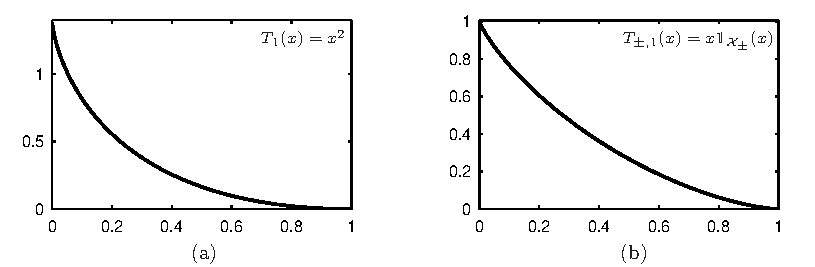
\includegraphics[width=.9\textwidth]{PDF/MaxEnt_LogisticLaw}}
\caption{Entropy  functional  $\phi_{\mathrm{u}}$   derived  from  the  logistic
  distribution:  (a)~with  $T_1(x)  =   x^2$  and  (b)~with  $T_{\pm,1}(x)  =  x
  \un_{\X_\pm}(x)$.}
%    ($c = \lambda_0 = 0, \lambda_1 = \overline{\lambda}_1 = -1$).}
\label{fig:Entropy-logistic}
\end{figure}



% ---------- Arcsine

\subsection{The arcsine distribution}
\label{subsec:Arcsine}

The arcsine distribution is a special case of the beta distribution with $\alpha
= \beta  = \frac12$. We  consider here the  centered and scaled version  of this
distribution which writes
%
\[
f_X(x) = \frac{1}{\pi\sqrt{ 2 \, \sigma^2 - x^2}} \qquad \mbox{on} \qquad \X = \left(
- \sigma \sqrt2 \, ; \, \sigma \sqrt2 \right).
\]
%
The inverse distributions $f_{X,\pm}^{-1}$ on $\X_-  = \left( - \sigma \sqrt2 \,
; \, 0 \right)$ and $X_+ = \left[ 0 \, ; \, \sigma \sqrt2 \right)$ write then
%
\[
f_{X,\pm}^{-1}(y) = \pm \frac{\sqrt{2 \pi^2  \sigma^2 y^2 - 1}}{\pi y}, \qquad y
\ge \frac{1}{\pi \sigma \sqrt2}
\]


Let us  now consider again  either a second  order moment as the  constraint, or
(partial) first order moment(s).


% -- Arcsine - second order

\subsubsection{Second order moment}

When  the second order  moment $T_1(x)  = x^2$  is constrained,  one immediately
obtains
%
\[
\phi'(y)=\lambda_0 + \lambda_1\left(2\sigma^{2}-\frac{1}{\pi^{2}y^{2}}\right)
\]
%
The family of entropy functional is then 
%
\[
\phi(y)  = c  +  \left( \lambda_0  +  2 \sigma^2  \lambda_1 \right)  y  \, +  \,
\frac{\lambda_1}{\pi^2 y}
\]
%
which    drastically   simplifies    with    the   special choice
%
\[
c  = 0,  \qquad \lambda_0  = -  \frac{\alpha^2}{\pi^2} \qquad  \mbox{and} \qquad
\lambda_1 = \pi^2 \qquad \mbox{to} \qquad\phi(y) = \frac{1}{y}
\]
%
% function   that   can   then    be   defined   over   which   is   represented
% figure~\ref{fig:Entropy-arcsin-var} for $\sigma=1$.


% ---------- Arcsine first order

\subsubsection{(Partial) first-order moment(s)}

Since the  distribution does not share the  sense of variation of  $T_1(x) = x$,
either we turn out to consider it as an extremal distribution of an entropy that
is not concave, or as a maximum entropy when constraints are of the type
%
\[
T_{\pm,1}(x) = x \un_{\X_\pm}(x)
% \quad \mbox{over} \quad \X_- = \left( - \sigma \sqrt2 \, ; \, 0
%\right), \quad \mbox{and} \quad \X_+ = \left[ 0 \, ; \: \sigma \sqrt2 \right).
\]
%
now 
%
\[
\phi_\pm'(y) = \sqrt2 \pi \sigma \lambda_0 + \lambda_{\pm,1} \frac{\sqrt{2 \pi^2
    \sigma^2  y^2 -  1}}{y} \qquad  \mbox{or} \qquad  \widetilde{\phi}_\pm'(y) =
\lambda_0 \pm \lambda_1 \frac{\sqrt{2 \pi^2 \sigma^2 y^2 - 1}}{y}
\]
%
where  the  different  factors  and  the  sign  are  absorbed  in  the  factors
$\lambda_0, \lambda_{\pm,1}$. A judicious choice can be to impose
%
\[
\lambda_{-,1} = \lambda_{+,1} = \overline{\lambda}_1 > 0
\]
%
and the  same integration constant $c$  for each branch, leading  then either to
the family of (convex)  uniform of functions $\phi(y) = \phi_{\mathrm{u}}(\sqrt2
\pi \sigma y)$ with
%
\[
\phi_{\mathrm{u}}(u) = c \, + \,  \lambda_0 \, u \, + \, \overline{\lambda}_1 \,
\left( \sqrt{u^2  - 1}  \, + \,  \arctan\left( \frac{1}{\sqrt{u^2 -  1}} \right)
\right) \un_{\left( 1 \, ; \, +\infty \right)}(u)
\]
%
or,  in  the  non-convex  case,   to  the  family  of  functions  with  branches
$\widetilde{\phi}_{\pm}(y) = \widetilde{\phi}_{\pm,\mathrm{u}}(\sqrt2 \pi \sigma
y)$,
%
\[
\widetilde{\phi}_{\pm,\mathrm{u}}(u) = c \, + \, \lambda_0 \, u \, \pm \, \lambda \, \left(
  \sqrt{u^2 - 1} \, +  \, \arctan\left( \frac{1}{\sqrt{u^2 - 1}} \right) \right)
\un_{\left( 1 \, ; \, +\infty \right)}(u)
\]


The      uniform      function      $\phi_{\mathrm{u}}$      is      represented
figure~\ref{fig:Entropy-arcsin}  for the  special  choice $c  =  \lambda_0 =  0,
\overline{\lambda}_1 = 1$  (here again, for $c = \lambda_0 =  0, \lambda_1 = 1$,
$\widetilde{\phi}_\pm = \pm \phi$).  In  this case again, the symmetrical choice
for  $\lambda_{\pm,1}$  allows to  recover  the  symmetries  of the  probability
density, and thus to a uniform convex entropy functional in the first context.

\
 
\begin{figure}[htbp]
\centerline{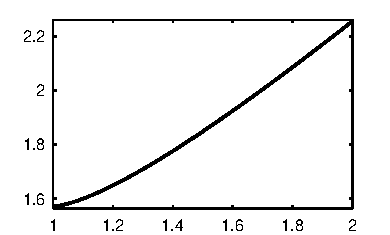
\includegraphics[width=.43\textwidth]{PDF/MaxEnt_ArcsineLaw}}
\caption{Entropy  functional   $\phi_{\mathrm{u}}$  derived  from   the  arcsine
  distribution with partial constraints $T_{\pm,1}(x) = x \un_{\X_\pm}(x)$.}
\label{fig:Entropy-arcsin}
\end{figure}


% ---------- Gamma first order

\subsection{The gamma distribution and (partial) $p$-order moment(s)}

\label{subsec:GammaFirstOrder}

As a very special case, consider here this distribution, expressed
as
%
\[
f_X(x) = \frac{\beta^\alpha  x^{\alpha-1} \exp(-\beta x)}{\Gamma(\alpha)} \qquad
\mbox{on} \qquad \X = \Rset_+.
\]
%
Let  us concentrate  on the  case $\alpha  > 1$  for which  the  distribution is
non-monotonous, unimodal, where the mode is located at $x = x_{\mathrm{m}}$, and
$f_X(\Rset_+) = \left[ 0 \, ; \, \frac1{\tau \,e^{\alpha-1}} \right]$ with
%
\[
x_{\mathrm{m}}  =   \frac{\alpha-1}{\beta}  \qquad  \mbox{and}   \qquad  \tau  =
\frac{\Gamma(\alpha)}{\beta \, (\alpha-1)^{\alpha-1}}
\]
%
Thus, here again it cannot be  viewed as a maximum entropy constraint neither by
any $p$-order  moment.  Here,  we can  again interpret it  as a  maximum entropy
constrained by partial moments
%
\[
T_{k,1}(x) = x^p, \quad k \in \{ 0  , -1 \} \qquad \mbox{over} \qquad \X_0 = [ 0
\, ; \, x_{\mathrm{m}} ) \qquad  \mbox{and} \qquad \X_{-1} = [ x_{\mathrm{m}} \,
; \: +\infty ).
\]
%
or as an extremal entropy constrained by the moment 
%
\[
T_1(x) = x^p \quad \mbox{over} \quad \X = \Rset_+
\]
%
where $p > 0$. Inverting $y = f_X(x)$ leads to the equation
%
\[
-  \frac{x}{x_{\mathrm{m}}} \exp\left(  - \frac{x}{x_{\mathrm{m}}}  \right)  = -
(\tau  \,  y )^{\frac{1}{\alpha -  1}}
%  \qquad  \mbox{with}  \qquad \tau  =  \left(
%  \frac{\Gamma(\alpha)}{\beta                              (\alpha-1)^{\alpha-1}}
%\right)^{\frac{1}{\alpha-1}}
\]
%
to be solved. As expected, this  equation has two solutions. These solutions can
be  expressed   via  the   multivalued  Lambert-W   function  $\W$   defined  by
$z=\W(z)\exp(\W(z))$,  i.e., $\W$  is  the  inverse function  of  $u \leadsto  u
\exp(u)$\cite[\S~1]{CorGon96}, leading to the inverse functions
\[
f_{X,k}^{-1}(y) = - x_{\mathrm{m}}  \, \W_k\left( - (\tau y)^{\frac{1}{\alpha
      - 1}} \right), \qquad y \in \left[ 0 \, ; \, \frac{1}{\tau e^{\alpha - 1}}
\right],
\]
%
where  $k$  denotes  the branch  of  the  Lambert-W  function. $k=0$  gives  the
principal branch and here it is related  to the entropy part on $\X_0$, while $k
= -1$ gives the secondary branch, related to $\X_{-1}$ here.

One has thus to solve the equation
%
\[
\phi'_k(y) =  \lambda_0 \tau  + \lambda_{k,1} \tau  \left[ - \W_k\left(  - (\tau
    y)^{\frac{1}{\alpha - 1}} \right) \right]^p
\]
%
where the  positive factor  are absorbed in  the $\lambda_0,  \lambda_{k,1}$ and
where to insure the convexity of the $\phi_k$,
%
\[
(-1)^k \lambda_{k,1} > 0
\]
%
The  same  approach  allows  to   design  $\widetilde{\phi}_k$,  with  a  unique
$\lambda_1$ instead of the $\lambda_{k,1}$.  Integrating the previous expression
is   not  an   easy   task.   Relation   $u  \,   (1+\W_k(u))   \,  \W_k'(x)   =
\W_k(u)$~\cite[Eq.~3.2]{CorGon96} suggests that a way to make the integration is
to    search   for    $\phi_k(y)    =    \phi_{k,\mathrm{u}}(\tau   y)$    where
$\phi_{k,\mathrm{u}}(u)$ is searched  as the product of $u  \left[- \W_k\left( -
  u^{\frac{1}{\alpha-1}}  \right)  \right]^p  $  and   a  series  of  $\left[  -
  \W_k\left( - u^{\frac{1}{\alpha-1}} \right) \right]$ and then to recognize the
coefficients of  the series. Such  an approach leads  to the family  of entropic
functional $\phi_k(y) = \phi_{k,\mathrm{u}}(\tau y)$ with
%
\[\begin{array}{l}
\phi_{k,\mathrm{u}}(u) \: = \: c_k + \lambda_0 \, u\\[2mm]
%
\hspace{7.5mm} + \, \lambda_{k,1} \, u \left[ - \W_k\left(
    -   u^{\frac{1}{\alpha-1}}   \right)  \right]^p   \left[   1  -
  \frac{p}{p+\alpha-1} \,  \, \hypgeom{1}{1}\left(  1 \, ;  \, p+\alpha \,  ; \,
    (1-\alpha)  \W_k   \left(  -  u^{\frac{1}{\alpha-1}}  \right)
  \right) \right] \un_{\left( 0 \, ; \, e^{1-\alpha} \right)}(u)
\end{array}\]
%
where   $\hypgeom{1}{1}$  is   the   confluent   hypergeometric  (or   Kummer's)
function~\cite[\S~13]{AbrSte70}  and $c_k$  are integration  constants. One  can
verify  a posteriori  that  these functions  are  the ones  we  search for.  The
integration constant
% (the  positive  multiplicative factor  is
%absorbed in the $\lambda_{k,1}$).  $\X_{-1}$ being unbounded, $c_{-1}$ is chosen
%to  be zero  and  $c_0$ 
can be chosen such that $\phi_k$ coincide in 0 for instance, that gives
%
\[
%c_0 = 0 \qquad \mbox{and} \qquad  
c_{-1} - c_0 \,  = \, \frac{p \, \Gamma(p+\alpha-1)}{(\alpha-1)^{p+\alpha-1}} \,
\lambda_{-1,1}
\]
%
using successively~\cite[Eq.~3.1]{CorGon96}  and~\cite[Eq.~13.1.2]{AbrSte70} for
$\W_0$,  and  successively~\cite[Eq.~13.1.4]{AbrSte70}   ($\W_{-1}$  tending  to
$-\infty$ in  $0^{-}$), $\W_{-1}(u) \exp(\W_{-1}(u)) =  u$, and~\cite[Eq.~4.6 \&
  lines that  follow]{CorGon96} for  $\W_{-1}$.  The same  algebra leads  to the
same expression  for the  $\widetilde{\phi}_k$, except that  $\lambda_{k,1}$ are
replaced by a unique $\lambda_1$.

The  multivalued   function  $\phi_{\mathrm{u}}$  in  the   concave  context  is
represented figure~\ref{fig:Entropy-gamma} for $p = 2, \alpha = 2$ and $\alpha =
5$,  and  with  the  choices  $c_{-1}  =  \lambda_0  =  0,  \lambda_{0,1}  =  1,
\lambda_{-1,1} = - 0.1$.
%
\begin{figure}[htbp]
\centerline{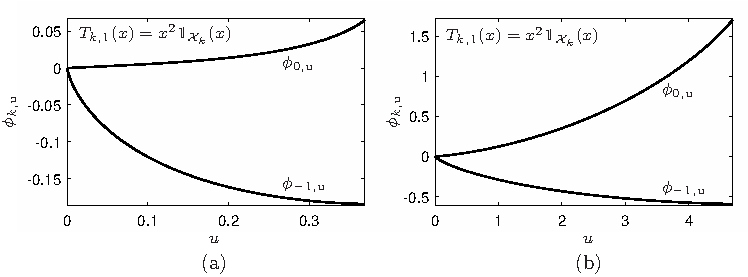
\includegraphics[width=.9\textwidth]{PDF/MaxEnt_GammaLaw}}
\caption{Multiform entropy functional $\phi_{\mathrm{u}}$ derived from the gamma
  distribution   with  the   partial  moment   constraints  $T_{k,1}(x)   =  x^2
  \un_{\X_k}(x)$, $k\in\{0,-1\}$.  (a): $\alpha = 2$; (b): $\alpha = 5$.}
%
\label{fig:Entropy-gamma} 
\end{figure}

\bibliographystyle{unsrt}
\bibliography{New_entropies}
\end{document}
